\documentclass[10pt]{beamer}

\usepackage[T2A]{fontenc}
\usepackage[utf8]{inputenc}
\usepackage[russian]{babel}
\usepackage{multicol}
\usepackage{hyperref}
\usepackage{caption}
\usepackage{subcaption}
\setbeamertemplate{navigation symbols}{} %отключение значков
\setbeamertemplate{caption}[numbered]
\usetheme{Warsaw}
\setbeamertemplate{footline}{%
    \hspace{0.94\paperwidth}%
    \usebeamerfont{title in head/foot}%
    \insertframenumber\,/\,\inserttotalframenumber%
}
\newcommand{\pdiff}[2]{\frac{\partial #1}{\partial #2}}
\newcommand{\op}[1]{\mathop{\mathrm{#1}}}
\graphicspath{{pictures/}}
\begin{document}

\title{Тестер ведомых SPI устройств}
\author{Студент гр. 506: Вебер Д.С.\\Руководитель:  ст.пр. Уланов П.Н.}
\date{2023}
\institute{Алтайский государственный университет}


\frame{\titlepage}

\begin{frame}{Цель и задачи}
  \textbf{Цель работы:} создать макет тестера ведомых устройств, работающих
по SPI интерфейсу.

  \textbf{Задачи:} 
  \begin{enumerate}
  \item Выбрать инструменты для разработки программы.
  \item Разработать программу.
  \item Собрать макет.
  \item Проверить работоспособность.
  \end{enumerate}
\end{frame}

\begin{frame}{Коротко о SPI}
  \begin{figure}
  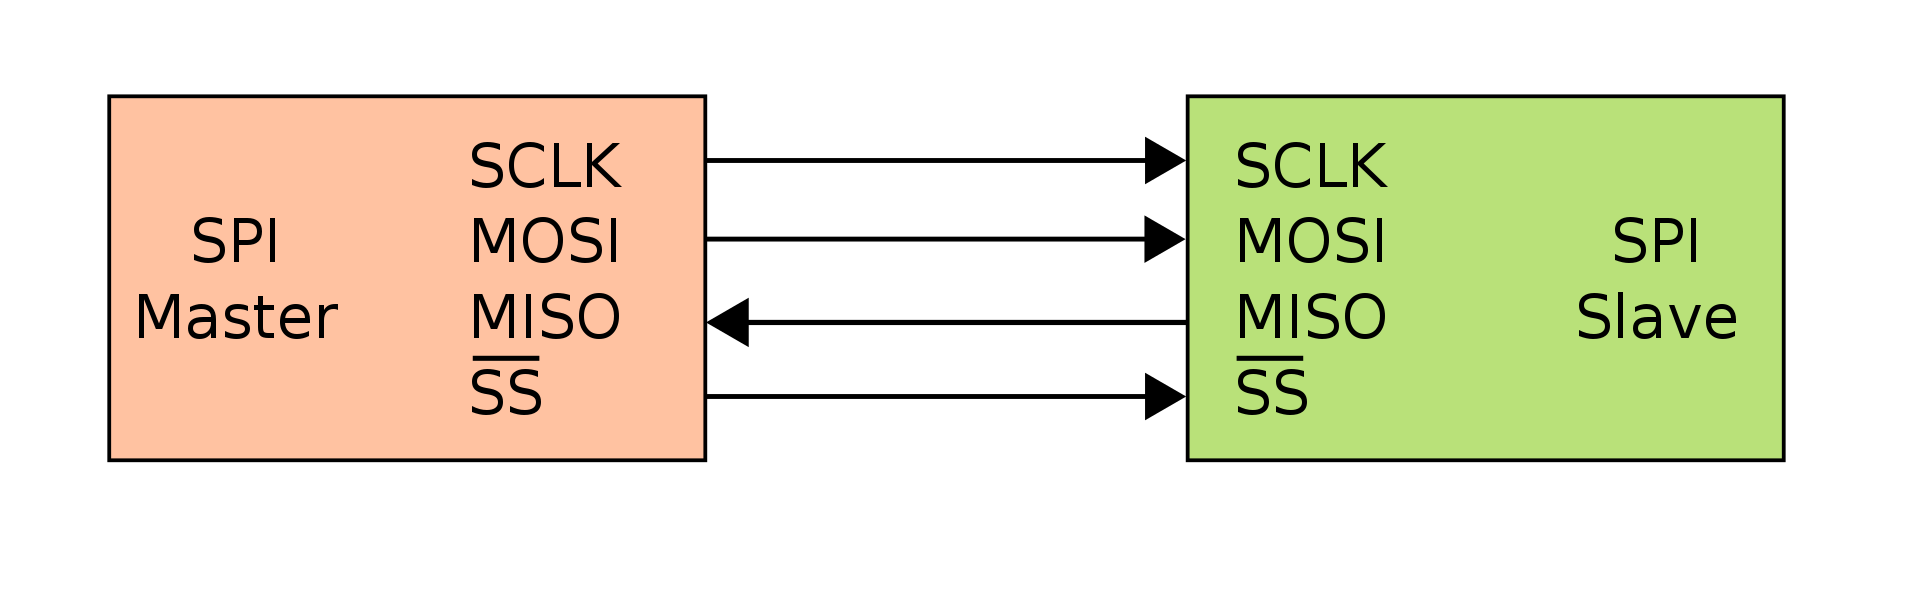
\includegraphics[width=0.9\textwidth]{spi}
  \caption{Ведущее (Master) и ведомое (Slave) устройства интерфейса SPI.}
  \end{figure}
\begin{footnotesize}
  		Интерфейс SPI поддерживает четыре режима работы, которые различаются настройками фазы (CPHA) и полярности (CPOL) сигнала тактирования:
	\begin{enumerate}
		\item Режим 0 (CPOL = 0, CPHA = 0): тактовый сигнал в низком уровне, выборка данных по переднему фронту.
		\item Режим 1 (CPOL = 0, CPHA = 1): тактовый сигнал в низком уровне, выборка данных по заднему фронту.
		\item Режим 2 (CPOL = 1, CPHA = 0): тактовый сигнал в высоком уровне, выборка данных по переднему фронту.
		\item Режим 3 (CPOL = 1, CPHA = 1): тактовый сигнал в высоком уровне, выборка данных по заднему фронту.
	\end{enumerate}
\end{footnotesize}
\end{frame}


\begin{frame}{Создание макета устройства}
  \begin{figure}
  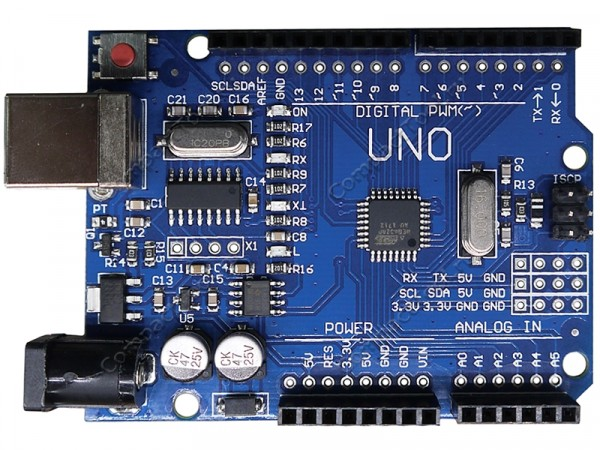
\includegraphics[width=0.5\textwidth]{uno}
  \caption{Arduino UNO.}
  \end{figure}
  Характеристики:
  \begin{itemize}
	\item Напряжение питания: 5 В.
	\item Цифровые входы/выходы: 14 линий.
	\item Аналоговые входы: 6.
	\item Flash-память: 32 Кб.
	\item Оперативная память: 2 Кб.
	\item Встроенные интерфейсы: i2c, spi, uart, usb.
  \end{itemize}
\end{frame}

\begin{frame}{Создание макета устройства}
  \begin{figure}
  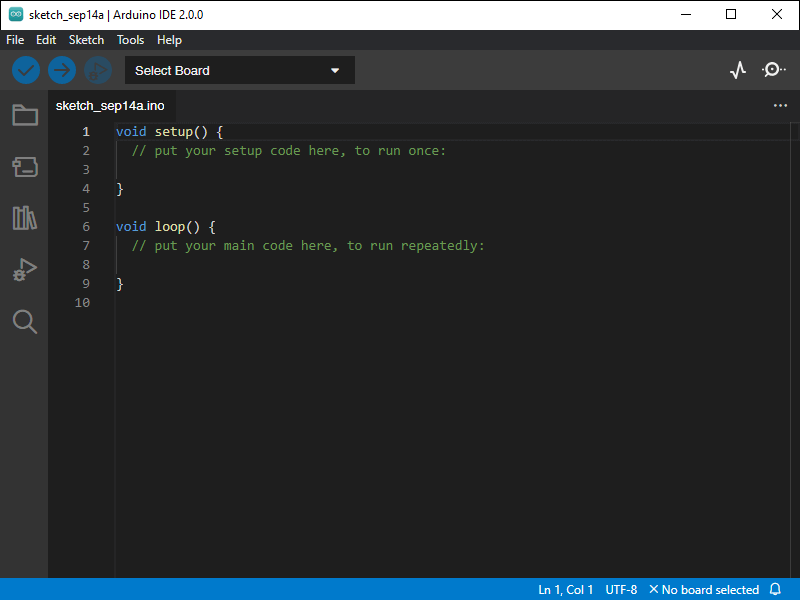
\includegraphics[width=0.9\textwidth]{ide}
  \caption{Arduino IDE.}
  \end{figure}
\end{frame}

\begin{frame}{Создание макета устройства}
Для разработки программы были использованы следующие библиотеки:
  \begin{enumerate}
  \item SPI.
  \item Keypad.
  \item OLED\_I2C.
  \end{enumerate}
\end{frame}

\begin{frame}{Создание макета устройства}
  \begin{figure}
  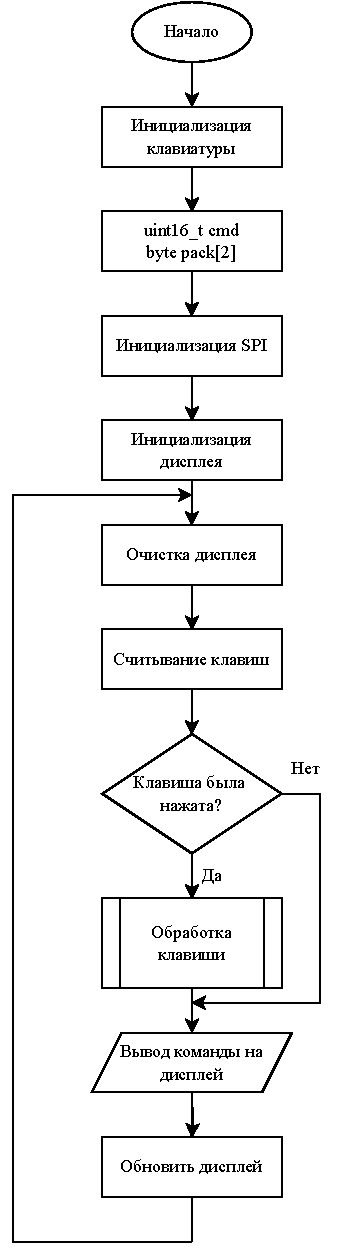
\includegraphics[width=0.2\textwidth]{main}
  \caption{Блок-схема главной программы.}
  \end{figure}
\end{frame}

\begin{frame}{Создание макета устройства}
  \begin{figure}
 	 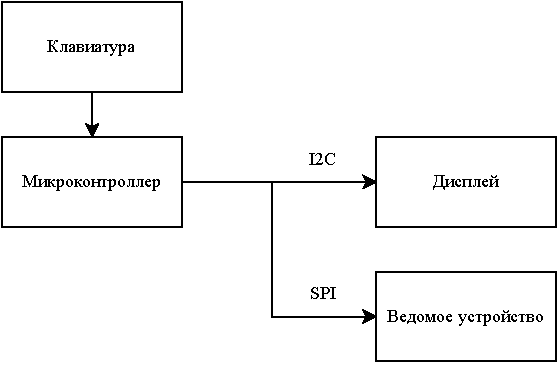
\includegraphics[width=1\textwidth]{scheme}
 	 \caption{Функциональная схема SPI тестера.}
  \end{figure}
\end{frame}

\begin{frame}{Описание работы устройства}
  \begin{figure}
 	 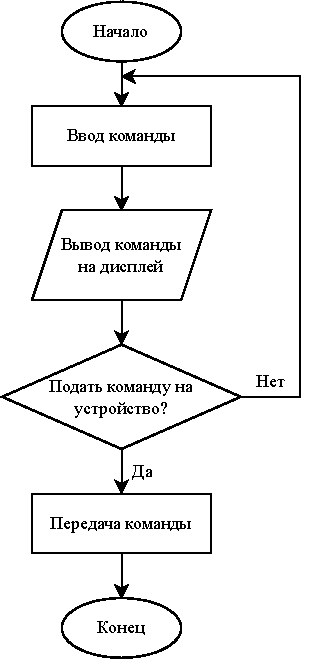
\includegraphics[width=0.35\textwidth]{struct}
 	 \caption{Структурная схема работы устройства.}
  \end{figure}
\end{frame}

\begin{frame}{Описание работы устройства}
\begin{figure}
\centering
\begin{subfigure}[t]{0.45\textwidth}
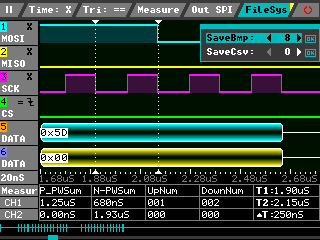
\includegraphics[width=1\textwidth]{testfreq}
\caption{Частота синхросигнала}
\end{subfigure}
\hfill     
\begin{subfigure}[t]{0.45\textwidth}
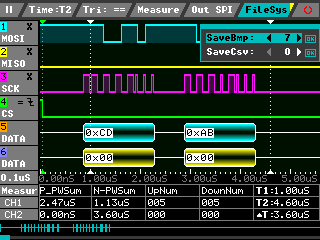
\includegraphics[width=1\textwidth]{test2}
\caption{0xABCD}
\end{subfigure}    
\caption{Данные с анализатора.}
\end{figure}
\end{frame}

\begin{frame}{Заключение}
	В результате научно-исследовательской работы были выполнены следующие задачи:
  \begin{enumerate}
  \item Выбраны инструменты для разработки программы.
  \item Разработана программа.
  \item Собран макет.
  \item Проверена работоспособность. 
  \end{enumerate}
  
 	По итогам работы цель достигнута: создан рабочий макет тестера ведомых SPI устройств.
\end{frame}

\end{document}
